\section{Gestione delle collection}

	\subsection{Visualizzazione dashboard} %UCU 8
	\label{visualizzazionedashboard}
	La dashboard è la pagina principale dalla quale è possibile avere accesso alla lista delle \glossario{collection} presenti nel sistema e alle altre funzionalità. Per accedervi è necessario aver eseguito l'autenticazione (vedi \ref{autenticazione}).

	\begin{figure}[H]
	\label{fig:dashboard}
		\centering 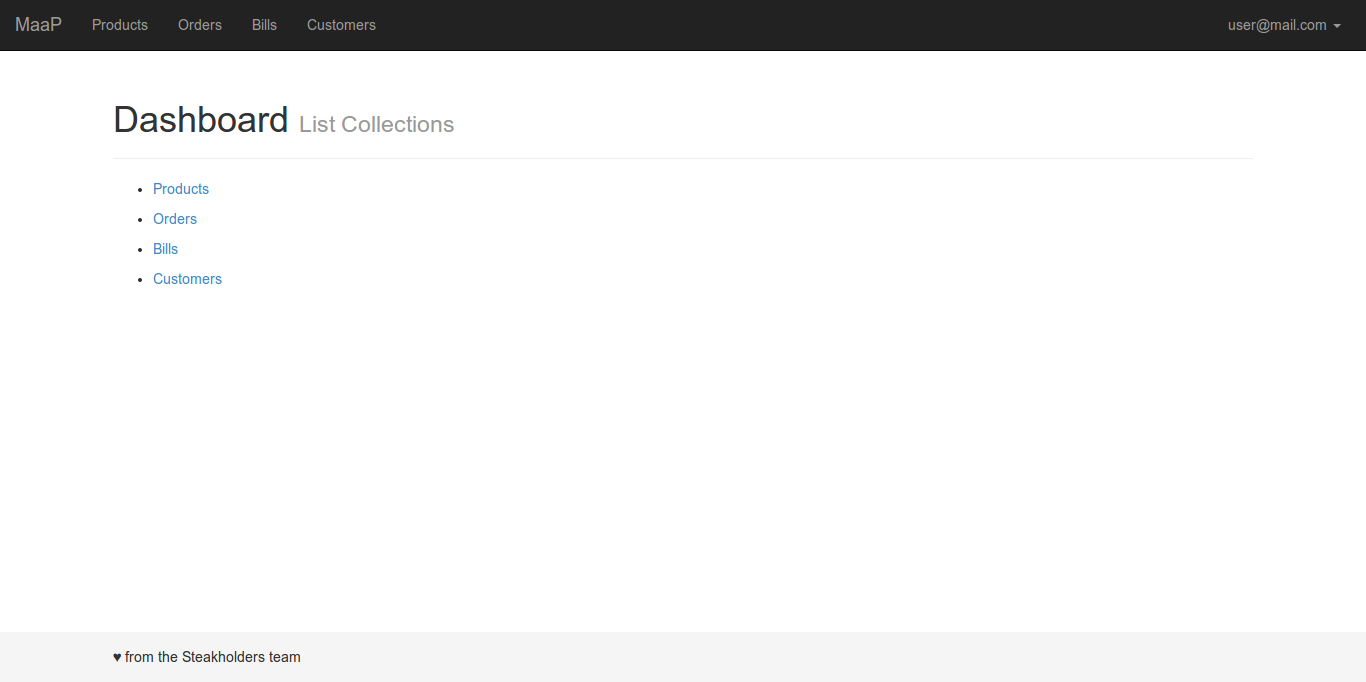
\includegraphics[width=1\textwidth]{img/dashboard.png}
	\caption{Pagina della dashboard}
	\end{figure}
	

	\subsection{Apertura collection index} %UCU 9
	\label{aperturacollectionindex}
	La \glossario{collection} index è la pagina in cui viene visualizzato il contenuto di una \glossario{collection} in forma tabellare. Per aprire una \glossario{collection} index (vedi figura \ref{fig:collection}) è necessario cliccare sul relativo link presente nella barra dei menù (1), MaaP visualizzerà l'intero contenuto della \glossario{collection} (2). La tabella visualizza i documenti dei quali è possibile aprire la showpage (vedi \ref{aperturashowpage}) cliccando sui relativi link (3). %TODO \`E possibile filtrare i contenuti della pagina tramite il pannello situato sulla destra.

	\begin{figure}[H]
		\centering 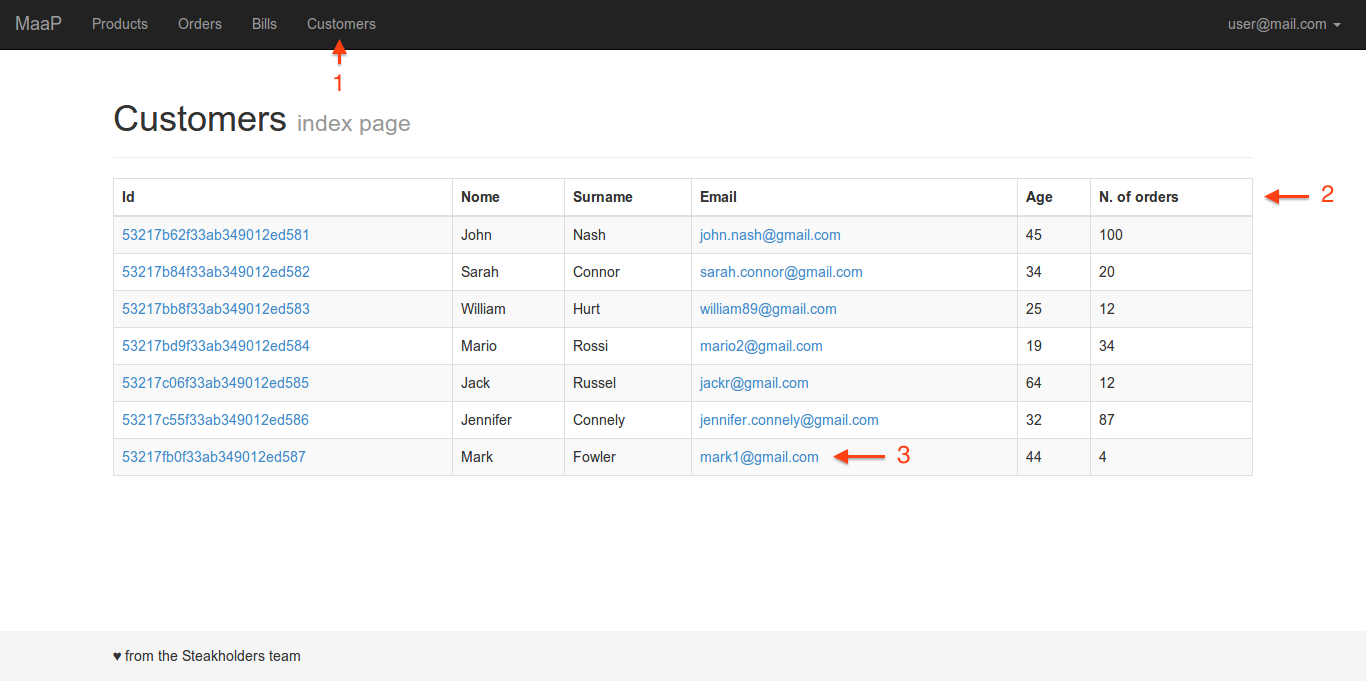
\includegraphics[width=1\textwidth]{img/collection.png}
	\caption{ \label{fig:collection} Index di una collection}
	\end{figure}
	

	\subsection{Apertura della show-page di un document} %UCU 9.
	\label{aperturashowpage}
	La show-page di un \glossario{document} visualizza gli attributi del documento in forma tabellare. Per accedere ad una show page è necessario posizionarsi nella \glossario{collection} index di appartenenza (vedi \ref{aperturacollectionindex}) e seguire il punto 3.

	\begin{figure}[H]
	\label{fig:showpage}
		\centering 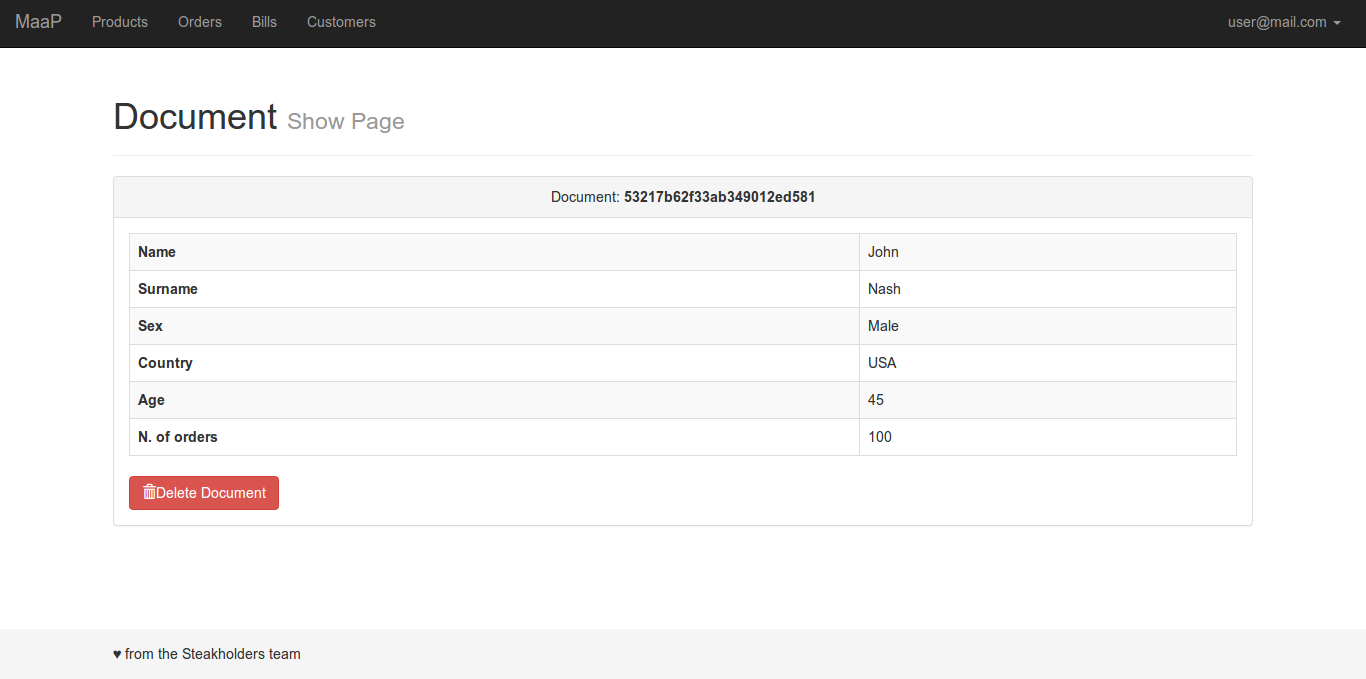
\includegraphics[width=1\textwidth]{img/showpage.png}
	\caption{Show page di un documento}
	\end{figure}

	\subsection{Visualizzazione show page attributi innestati} % 9.1.1
	La presenza di \glossario{document} innestati viene evidenziata dalla visualizzazione dell'attributo come un link, attraverso il quale è possibile accedere alla show page. 


	%\subsection{Filtra risultati} %TODO viene implementato in RA
